\documentclass[main.tex]{subfiles} 

\begin{document}
%%%%%%%%%%%%%%%%%%%%%%%%%%%%%%%%%%%%%%%%%%%%%%%%%%%%%
%%%%%%%%%%%%%%%%    Appendices   %%%%%%%%%%%%%%%%%%%%
%%%%%%%%%%%%%%%%%%%%%%%%%%%%%%%%%%%%%%%%%%%%%%%%%%%%%
\appendix
\section*{Vedlegg 1 - Kartleggingsprøven i sannsynlighetsregning}
\label{prove}
Denne kartleggingsprøven (se neste side) ble brukt til å evaluere elever fra 10. trinn
i følgende kompetansemål 
\begin{itemize}
\item finne og diskutere sannsyn gjennom eksperimentering, simulering og berekning i daglegdagse samanhengar og spel
\item beskrive utfallsrom og uttrykkje sannsyn som brøk, prosent og desimaltal
\end{itemize}
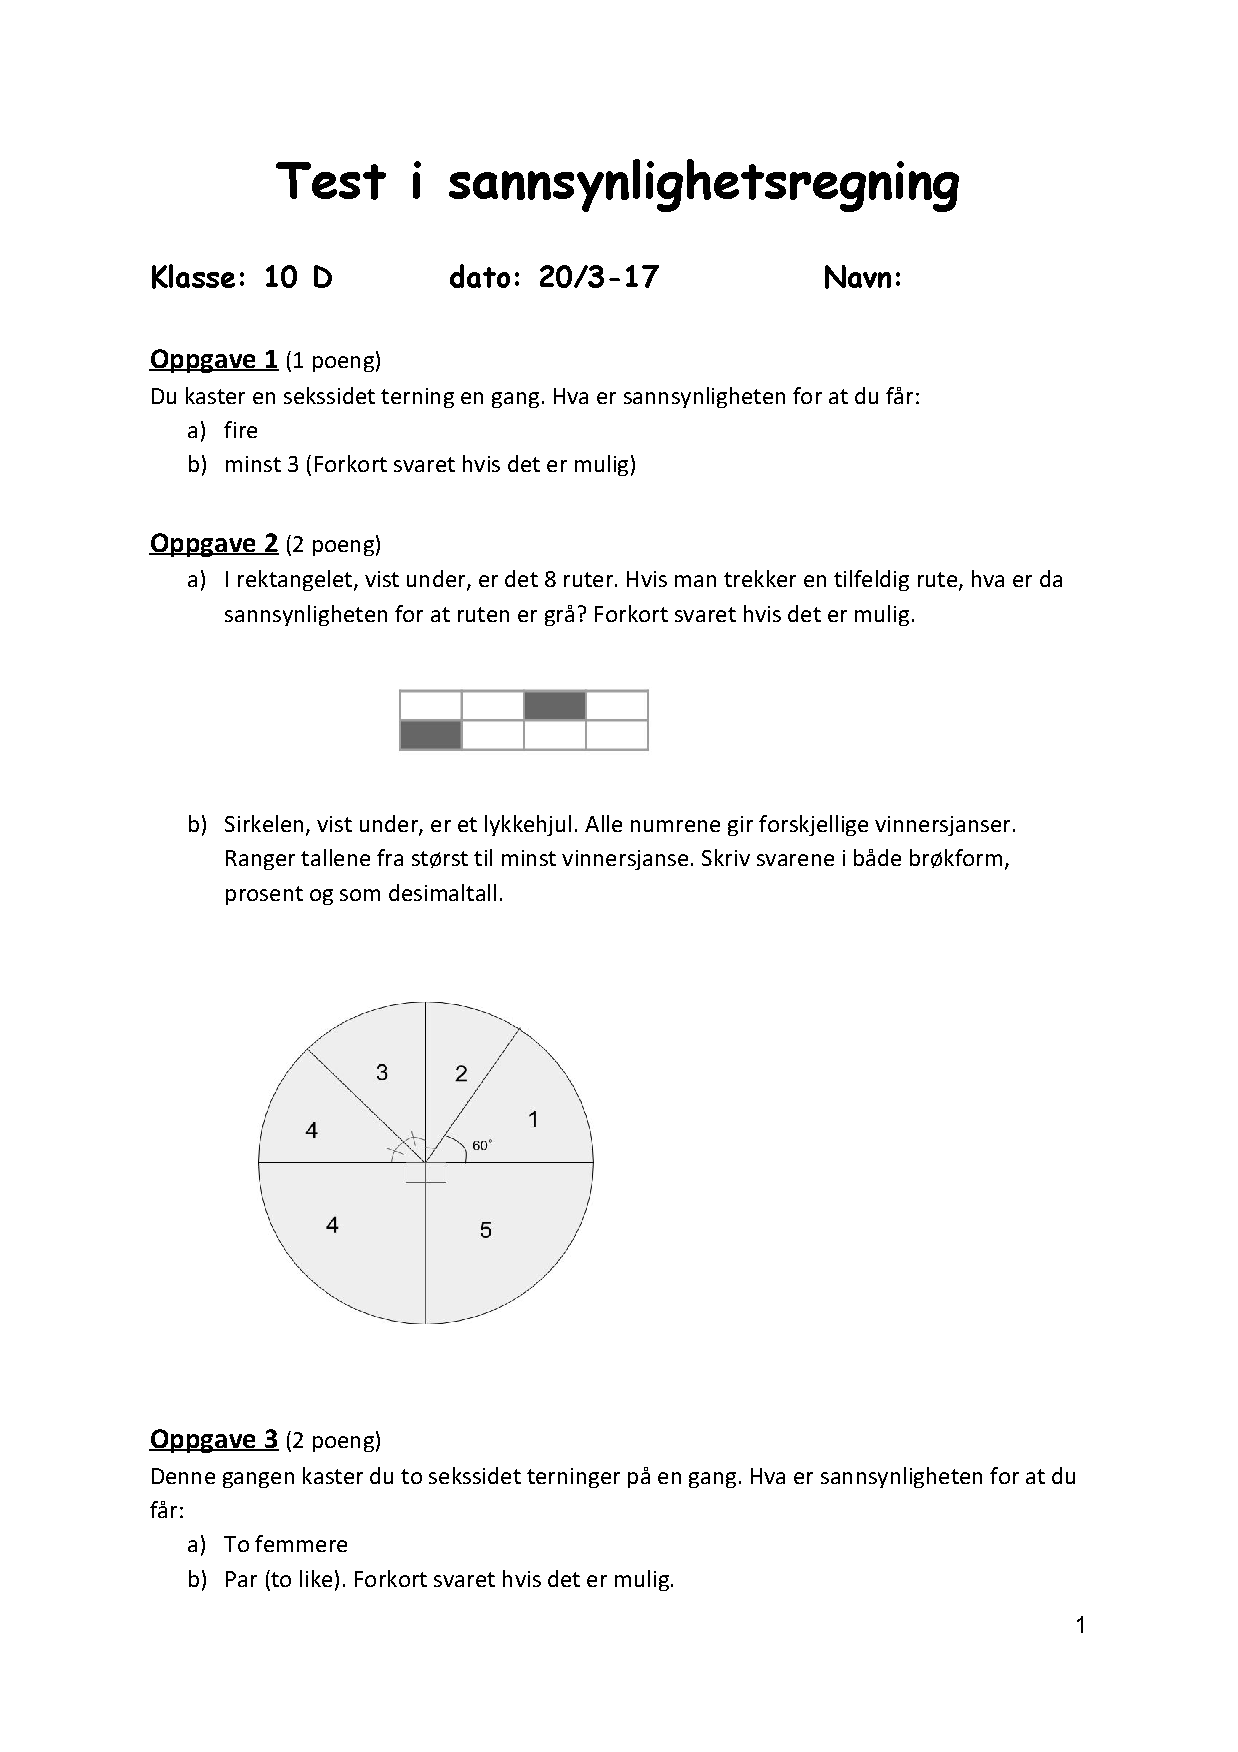
\includepdf[page = 1,scale = 0.9]{../figures/testen.pdf}
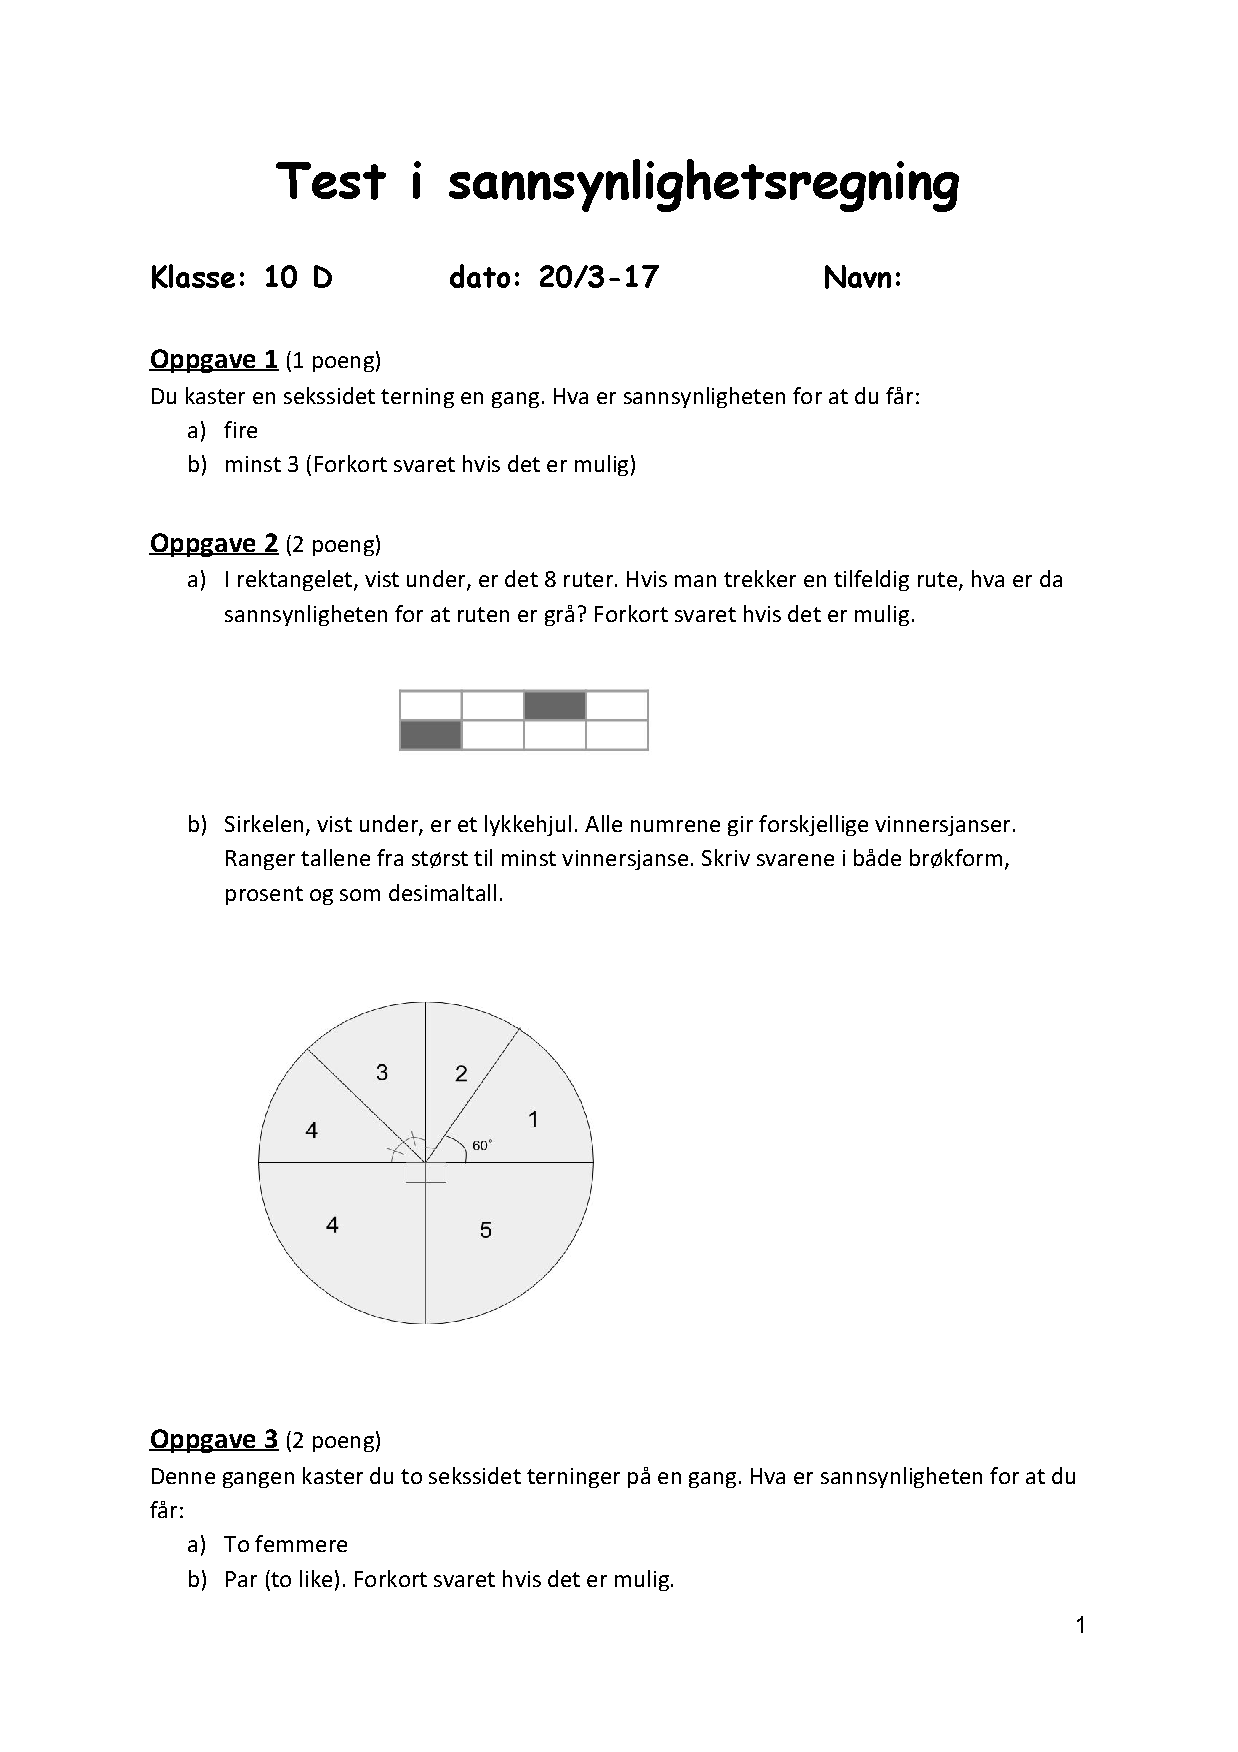
\includepdf[page = 2,scale = 0.9]{../figures/testen.pdf}

\end{document}
